\documentclass[a4paper,twoside]{articlewithlogo}

\usepackage{enumerate}
%\usepackage{enumitem}
\usepackage{graphicx}
\graphicspath{{Figuras/}}
\usepackage{color}
\usepackage[cmex10]{amsmath}
\usepackage{array}
\usepackage{float}
\usepackage{multicol}
\usepackage[utf8]{inputenc} 
\usepackage[T1]{fontenc}
\usepackage[french]{babel}
%\usepackage[font=normalsize,format=plain,labelfont=bf,up,textfont=up,figurename=Figura,tablename=Tabela]{caption}
\usepackage[tablename=Tableau]{caption}
\usepackage{subcaption}
\usepackage[top=1in, bottom=1in, left=1.25in, right=1.25in]{geometry}
\usepackage{indentfirst}
\usepackage{fancyhdr}
% Font packages
\usepackage{amssymb}
\usepackage{amsfonts}
\usepackage{pgfgantt}
\usepackage{steinmetz}
\usepackage{rotating}
% Nice extra font package, e.g. \mathds{1}
\usepackage{dsfont}
\usepackage{color}
\usepackage{blindtext}
% Use multiple rows when writing tables
\usepackage{multirow}
\usepackage{booktabs}
\usepackage{bm}
\usepackage{bigstrut}
% Uncomment next line to make footnots per page
\usepackage{perpage}
% Uncoment next group of lines to create the table of contents for the PDF
\usepackage{hyperref}
\usepackage[toc,page]{appendix}
\usepackage{listings}
\usepackage{currfile}

\definecolor{darkblue}{rgb}{0,0,0.5}
\definecolor{darkblue}{rgb}{0,0,0.5}
\renewcommand{\title}{Étude des régulations en tension des réseaux de distribution}
\newcommand{\subtitle}{Rapport d'activité de Stage 2A}

\hypersetup{
    pdftitle={\title},
    pdfauthor={Rafael Accacio Nogueira},
    bookmarksnumbered=true,     
    bookmarksopen=true,         
    bookmarksopenlevel=1,       
    colorlinks=true,
    linkcolor=black,
    filecolor=darkblue,  
    urlcolor=darkblue,  
    citecolor=darkblue,              
    pdfstartview=Fit,          
    pdfpagemode=UseOutlines,    % this is the option you were lookin for
    pdfpagelayout=TwoPageRight
}
\let\oldcontentsline\contentsline%
\renewcommand\contentsline[4]{%
    \oldcontentsline{#1}{\smash{\raisebox{1em}{\hypertarget{toc#4}{}}}#2}{#3}{#4}}

\newcommand\mysection[1]{\section[#1]{\protect\hyperlink{tocsection.\thesection}{#1}}\label{#1}}
\newcommand\mysubsection[1]{\subsection[#1]{\protect\hyperlink{tocsection.\thesection}{#1}}\label{#1}}
\newcommand\mysubsubsection[1]{\subsubsection[#1]{\protect\hyperlink{tocsection.\thesection}{#1}}\label{#1}}

\newcommand{\conteudo}{\tableofcontents\label{tocsection}}


\pagestyle{fancy}
\newif\ifdebug
\newcommand{\draft}{\debugtrue}
\newcommand{\final}{\debugfalse}
\newcommand\todo[1]{\ifdebug {\color{red}#1}\else \PackageError{}{FORGOT TO DO SOMETHING}{}\fi}
\newcommand\doing[1]{\ifdebug {\color{blue}#1}\fi}
\newcommand\warning[1]{\ifdebug {\color{red}#1}\fi}


\fancyhead[CO]{\title}
\fancyhead[CE]{\subtitle}
%\fancyhead[RE]{\rightmark}
\fancyhead[L]{\warning{DRAFT}}
\fancyhead[R]{\warning{DEBUG ON}}

\fancyfoot[L]{\warning{TURN DEBUG OFF}}
\fancyfoot[R]{\warning{DRAFT}}

\fancyfoot[C]{\thepage}

\allowdisplaybreaks

\usepackage{chngcntr}
\counterwithin{figure}{section}


\newcommand{\figplaceholder}[1]{\ifdebug
	\begin{figure}[H]
		\begin{center}	
			\rule{8cm}{8cm}
			\caption{\color{red}placeholder}
			\label{fig:#1}
		\end{center}
	\end{figure}
\else
\PackageError{}{NO FIGURE}{}
\fi
}


\usepackage[acronym]{glossaries}\makeglossaries
\newcommand{\acr}[3]{\newacronym{#1}{#2}{#3}}
\newcommand{\symbl}[3]{\newglossaryentry{#1}{name = #2,	description = #3,}}


\usepackage[acronym]{glossaries}
%
\newacronym{Supelec}{Supélec}{École Supérieure d'Électricité}
\newacronym{la}{LA}{Los Angeles}
\newacronym{un}{UN}{United Nations}
%
%
%% nomenclature:

%\newglossaryentry{numofangels}{
%	name = $N$ ,
%	description = The number of angels per needle point
%}
%\newglossaryentry{areaofneedle}{
%	name = $A$ ,
%	description = The area of the needle point
%}

\newcommand{\symbl}[3]{
\newglossaryentry{#1}{
	name = #2 ,
	description = #3,
}
}

\debugtrue
\makeglossaries
\makeindex
\begin{document}
\large
\renewcommand{\figurename}{Figure}
\todo{REMEMBER TO TURN DEBUG OFF}





%\begin{titlepage}
%\begin{center}
%% Upper part of the page. The '~' is needed because \\
%% only works if a paragraph has started.
%
\includegraphics[width=60mm]{logos/supelec.jpeg}%~\\[0.5cm]
%\vspace{50pt}
%% Title
%\rule{\linewidth}{0.5mm} \\[0.4cm]
%{ \huge \bfseries \title \\[0.4cm] }
%\rule{\linewidth}{0.5mm} \\[0.5cm]
%\textsc{\Large \subtitle}\\[1.5cm]
%\vspace{60pt}
%% Author and supervisor
%\begin{minipage}{0.4\textwidth}
%\center
%\normalsize
%{Rafael Accácio NOGUEIRA\vspace{50pt} }
%
%\large
%\textbf{Orienté par\\M. Hervé GUÉGUEN}
% \\
% \vspace{50pt}
% 
\includegraphics[width=60mm]{logos/logo_IETR_rvb.jpg}
%\end{minipage}
%\vfill
%
%% Bottom of the page
%{\large \today}
%\end{center}
%
%\teacher{M. Hervé GUÉGUEN}
%\end{titlepage}

\begin{titlepage}
	\begin{center}
		% Upper part of the page. The '~' is needed because \\
		% only works if a paragraph has started.
		\vspace{50pt}
		\begin{minipage}{\textwidth}
		\begin{minipage}{.4\textwidth}
		
\includegraphics[width=\textwidth]{logos/supelec.jpeg}%~\\[0.5cm]
		\end{minipage}
		\hspace{.2\textwidth}
		\begin{minipage}{.4\textwidth}
		
\includegraphics[width=\textwidth]{logos/logo_IETR_rvb.jpg}
		\end{minipage}
		\vspace{100pt}
		\end{minipage}
		% Title
		\rule{\linewidth}{0.5mm} \\[0.4cm]
		{ \huge \bfseries \title \\[0.4cm] }
		\rule{\linewidth}{0.5mm} \\[0.5cm]
		\textsc{\Large \subtitle}\\[1.5cm]
		\vspace{60pt}
		% Author and supervisor
		\begin{minipage}{0.4\textwidth}
			\center
			\large
			{Rafael Accácio NOGUEIRA\vspace{50pt} }
			
			\normalsize
			\textbf{Orienté par\\M. Hervé GUÉGUEN}
			\\
		\end{minipage}
		\vfill
		
		% Bottom of the page
		{\large \today}
	\end{center}
	
	\teacher{M. Hervé GUÉGUEN}
\end{titlepage}
\conteudo
\newpage
\mysection{Objectif}
L'objectif de ce document est faire un rapport du stage, qui détaille le lieu de travail, toutes les choses produits pendant le stage en expliquant les méthodes utilisés et qui montre les résultats obtenus, les commente et dit les implications des conclusions.
\mysection{Introduction Générale}
Afin de compléter la formation du 2A CentraleSupélec, un stage a été réalisé entre lesm ois de juillet et septembre de 2017, au sein du laboratoire de l'équipe \gls{AUT} du	
\gls{IETR} en travaillant au cadre du projet d'\title, avec la orientation de M. Hervé GUÉGUEN.


\mysubsection{Sur le lieu de travail} 
\mysubsubsection{L'IETR}
L'IETR est un institut de recherche français, spécialisé en électronique et télécommunication, localisé à Rennes, comptant avec plus que 300 enseignants-chercheurs, ingénieurs, doctorants et administratifs, il est formé par équipes de recherche des écoles et instituts de recherche de la région comme le CNRS, l'Université Rennes 1, INSA de Rennes, CentraleSupélec et Université de Nantes.

En relation aux partenariats avec autres instituts et entreprises, L'IETR a une liste considérable de partenaires, incluent des centres publiques comme CEA, CNES et Club Automatique et Automatisation industrielle de la SEE, petites et moyennes entreprises privés comme A\&P Lithos, Adlightec et Advansee, et grandes groupes comme Alstom, EDF et Mitsubishi. 

Son partenariat International compte sur plus de 70 Universités, Instituts et Agences de recherche parmi tout le monde, incluent \gls{JPL}, \gls{Polimi} et \gls{USP}.

\mysubsubsection{Division des Équipes de Recherche}
Afin de meilleur catégoriser les thématiques des projets de recherche L'IETR est divisé en 6 départements/équipes:

\begin{itemize}
	\item Antennes \& Dispositifs Hyperfréquences (ADH)
	\item Signal \& Communications (SC)
	\item Ondes \& Signaux (OS)
	\item Image
	\item Microélectronique \& Microcapteurs (MM)
	\item Automatique (AUT)
\end{itemize}

L'organigramme structurel avec tant les parties de recherche quant les parties administratifs du IETR peut être vu dans la figure \ref{fig:organigramme_IETR_160717_v28}.
\pagebreak
\mysubsubsection{L'équipe AUT}
L'équipe de Automatique est basé a CentraleSupélec et travaille dans diverses thématiques utilisant les connaissances des domaines de analyse et commande des systèmes hybrides, et ses projets ont des applications que couvrent diverses métiers, par exemple projets de bâtiments intelligents, santé, chimie, transport, distribution d'énergie ( métier du projet que j'ai réalisé ) entre autres.\\
\todo{Dar Exemplos de projetos e conferências 5 linhas}

\begin{figure}[H]
	\begin{center}	
		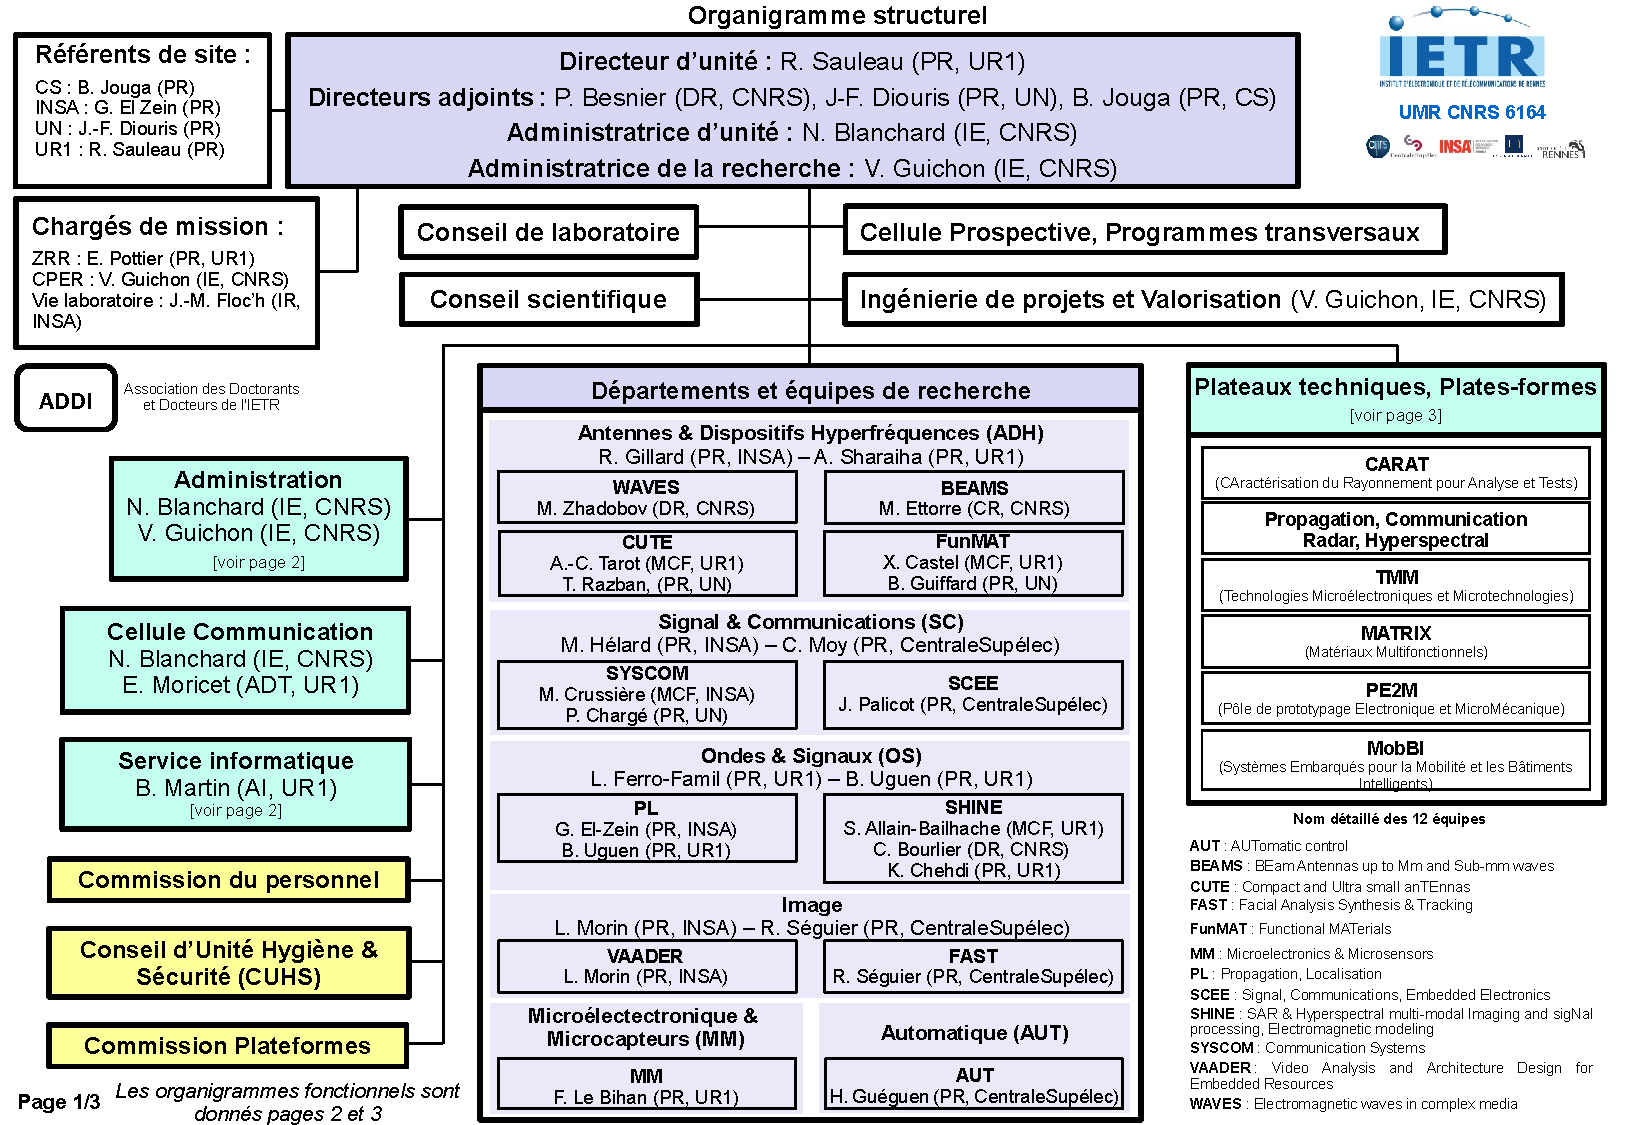
\includegraphics[width=\textwidth]{./organigramme_IETR_160717_v28.pdf}
		\caption{Organigramme du IETR.}
		\label{fig:organigramme_IETR_160717_v28}
	\end{center}
\end{figure}












  
\listoffigures
\listoftables
\section{Objectif}
\begin{frame}{Objectif du projet}



\end{frame}


\input{Méthodologie}
\section{Résultats}
\begin{itemize}
	\item 
\end{itemize}

\newpage
\mysection{Difficultés}
Pendant le projet quelques difficultés ont été trouvé et les principaux sont les suivantes:

\begin{itemize}
	\item Long temps de calcule\\
	Le modèle avec le régulateur implémenté dans simulink prend 5 min a peu près, quoi a difficulté le \textit{debuging} du système comme la génération des résultats.\\ 
	\item Touts blocs en PowerFactory sont synchrones\\
	Dû a ça, le filtres a été implémenté dehors simulink, augmentant la complexité du modèle, 4 blocs plus ont été crée.\\
	\item Conditions Initiales\\ 
	A cause des différents blocs utilisés chaque bloc avait besoin d'avoir ses conditions initiales cohérents entre elles, qui causait de problèmes cas elles ne fussent pas cohérents.\\
	\item Documentation du \powerfactory\\
	Documentation du logiciel n'est pas bien détaillé, causant quelquefois ambiguïté, créant le besoin de chercher l'information en autres lieux.\\
	\item Communauté PowerFactory presque inexistant\\
	Pour trouver des informations il fallait chercher a l'internet, mais la principale source était le faq du PowerFactory, qu'est si réticent quant la documentation. 
\end{itemize}

\mysection{Prochains Travails}
Pour prochains travails quelques choses peuvent être suggérées:
\begin{itemize}
	\item Implémenter un bloc dans PowerFactory que soit appelé en temps différent du pas de la simulation.
	\item Réduire temps de communication PowerFactory$ \leftrightarrows $Matlab
	\item Automatiser les diverses simulations et la génération des figures.
\end{itemize}
\newpage
\mysection{Conclusions}
On peut arriver a quelques conclusions après avoir vu toute le méthodologie utilisé et les résultats en graphiques et tableaux, et elles sont:

\begin{itemize}
	\item \textbf{Scripting en PowerFactory}\\
	Il est possible d'utiliser Python et la combinaison entre l'API PowerFactory avec les bibliothèques Python déjà crées permet une gamme de possibilités.\\
	\item \textbf{Intégration Matlab $\mathbf{\leftrightarrows }$ PowerFactory}\\
	Assez facile si toute les variables du système sont préalablement connues.\\
	\item \textbf{Stabilité dus système dépendent de la valeur de $ a $}\\
	Régulateur fonctionne mais dépend de $ a $ pour rester stable, valeurs plus proches de 1 font le système stabiliser plus vite.
	
\end{itemize}

\symbl{angelsperarea}{adazd}{anjos por area}
\gls{Supelec} 
%, \gls{la} and \gls{un} are abbreviations whereas
\gls{angelsperarea}
%, \gls{numofangels} and \gls{areaofneedle} are part of the
nomenclature



\Blindtext

\printglossary[type=\acronymtype,title=Liste des Acronymes]
%
\printglossary[title=Glossaire]
%\newpage
%\begin{appendices}
%	\input{Appendices/Communication}
%\end{appendices}
%\newpage
%\nocite{*}
%\bibliographystyle{plain}
%\bibliography{bibliografia}

\end{document}